\documentclass[12pt, a4paper]{article}
\usepackage{amsmath, amsthm, amssymb, appendix, bm, graphicx, hyperref,mathrsfs,fancyhdr,ctex,nameref,tikz,listings,xltxtra,float}


% 定义新的页眉样式
\fancypagestyle{sectionheader}{
    \fancyhf{} % 清空当前页眉设置
	\fancyhead[L]{Page:\thepage}
	%\fancyhead[C]{中间页眉}
	\fancyhead[R]{\leftmark}
}
\setlength{\headheight}{14.49998pt}
\addtolength{\topmargin}{-2.49998pt}


\numberwithin{equation}{section} % 每个节开始时重新编号公式
\title{Final Project of MathSoft}
\author{PhilFan}
\date{\today}
\linespread{1.5}


\begin{document}

\maketitle
\setcounter{page}{0}
\maketitle
\thispagestyle{empty}


%目录页
\newpage
\pagenumbering{Roman}
\setcounter{page}{1}
\tableofcontents

%第一节
\newpage
\setcounter{page}{1}
\pagenumbering{arabic}
\pagestyle{sectionheader} % 使用自定义的页眉样式


\section{流程}
123
\cite{refa}
根据这篇文档生成了以下的部分
生成了如下的结果\ref{pic}


\begin{figure}[H]% 插入一张图片,H表示浮动环境下的here
	\centering
	\begin{minipage}{0.83\textwidth}% 小页面尺寸,可自行调节
		\centering
		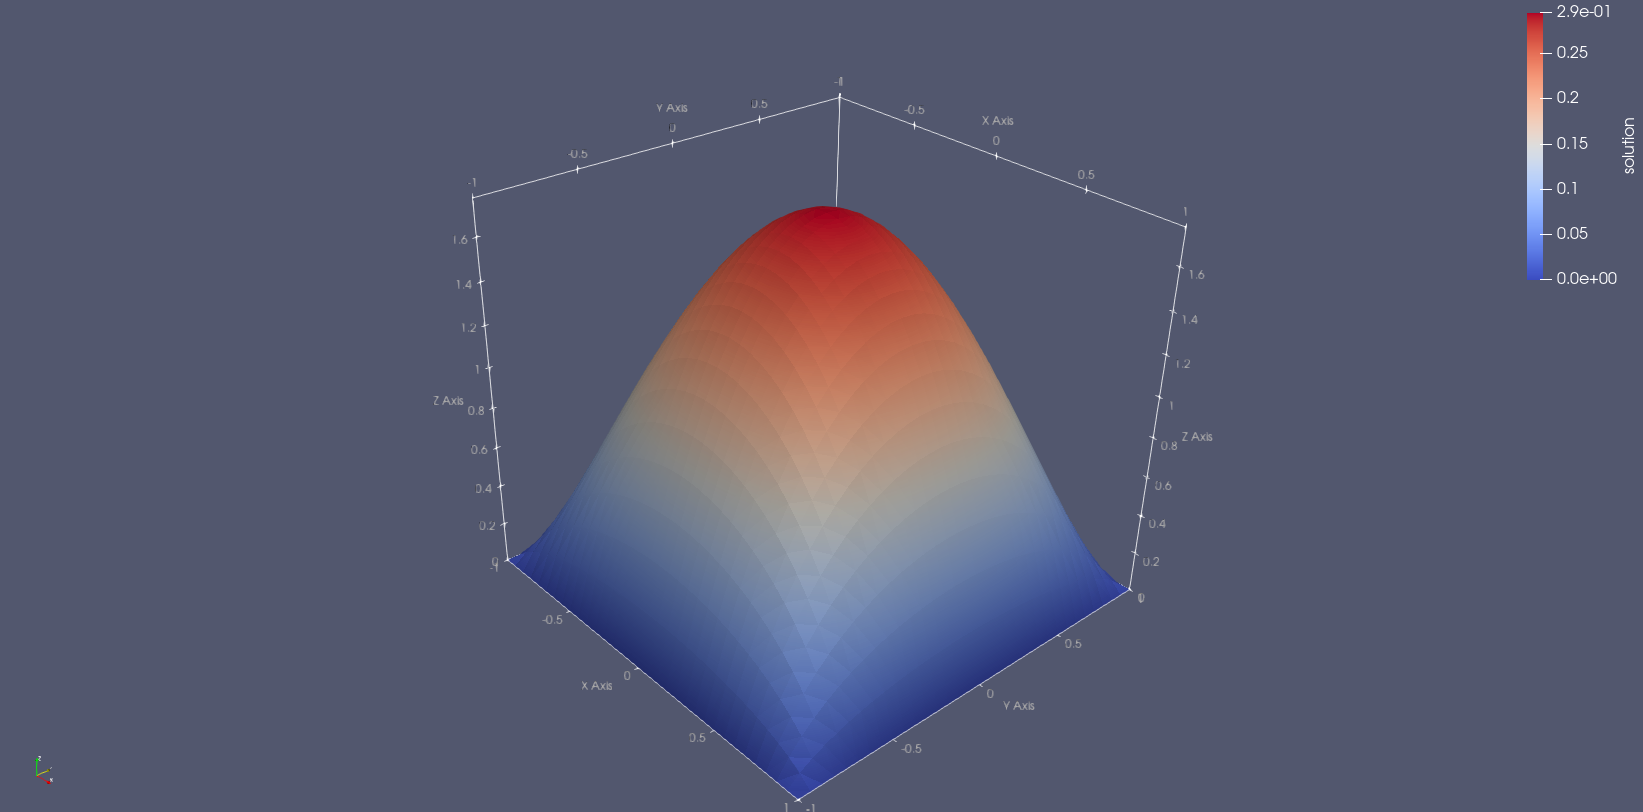
\includegraphics[width=1.0% 图片尺寸,可自行调节
		\textwidth]{proj.png}% 图片名称(图片需与tex文件在同一文件夹)
		\caption{\fontsize{10pt}{15pt}\selectfont 得到的结果}% 图例
		\label{pic}
	\end{minipage}
\end{figure}


\newpage
\section{有限元方法的基本设置}
这是我们实际使用有限元来计算某些东西的第一个示例。我们将求解一个边界值为零但右侧为非零的泊松方程的简单版本:

\begin{align*} 
	-\Delta u &= f 	\qquad 	\qquad & \text{in}\ \Omega,\\ 
	u &= 0 		\qquad	\qquad & \text{on}\ \partial\Omega. 
\end{align*}

我们将在正方形上求解这个方程,$\Omega=[-1,1]^2$,为此,您已经学会了如何在步骤 1 和步骤 2 中生成网格。在这个程序中,我们也将只考虑特殊情况$\Omega=[-1,1]^2$并回到如何在下一个教程程序 Step-4 中实现更一般的情况。

如果您已经了解了有限元方法的基础知识,您将记得我们需要采取的步骤来近似解u通过有限维近似。具体来说,我们首先需要推导出上述方程的弱形式,我们通过将方程乘以测试函数来获得$\varphi$ 从左边(我们将回到从左边乘法而不是从右边乘法的原因)并在域上积分$\Omega$:
\begin{align*} -\int_\Omega \varphi \Delta u = \int_\Omega \varphi f. \end{align*}
这可以通过部件进行集成:
\begin{align*} \int_\Omega \nabla\varphi \cdot \nabla u - \int_{\partial\Omega} \varphi \mathbf{n}\cdot \nabla u = \int_\Omega \varphi f. \end{align*}
测试功能$\varphi$必须满足相同类型的边界条件(用数学术语来说:它需要来自我们寻求解的集合的切空间),所以在边界上$\varphi = 0$因此,我们正在寻找的弱形式读取
\begin{align*} (\nabla\varphi, \nabla u) = (\varphi, f), \end{align*}

我们使用了通用符号的地方$(a,b)=\int_\Omega a\; b$一乙.然后问题要求一个函数$u$此语句适用于所有测试函数$u$从适当的空间(这里是空间$H^1$).

当然,在一般情况下,我们无法在计算机上找到这样的功能,而是寻求近似值$u_h(\mathbf x)=\sum_j U_j \varphi_j(\mathbf x)$,其中$U_j$是我们需要确定的未知膨胀系数(这个问题的“自由度”),以及$\varphi_i(x)$是我们将使用的有限元形状函数。要定义这些形状函数,我们需要以下内容:

用于定义形状函数的网格。您已经了解了如何在步骤 1 和步骤 2 中生成和操作描述网格的对象。
一个有限元,用于描述我们要在参考单元格上使用的形状函数(在 \verb|deal.II| 中始终是单位区间[0,1]、单位平方$[0,1]^2$或单位立方体$[0,1]^3$,具体取决于您工作的空间维度)。在步骤 2 中,我们已经使用了类型为\verb| FE\_Q<2>| 的对象,它表示通过在支撑点上插值来定义形状函数的常用拉格朗日元素。最简单的是\verb|FE\_Q<2>|(1),它使用多项式次数1。在 2d 中,这些通常称为\textit{双线性},因为它们在参考单元格的两个坐标中的每一个都是线性的。(在 1d 中,它们是线性的,在 3d 中是三线性的;但是,在 \verb|deal.II|文档中,我们通常不会进行这种区分,而只是简单地称这些函数为“线性”。

一个 \verb|DoFHandler| 对象,它枚举网格上的所有自由度,以有限元对象提供的参考单元格描述为基础。您还已经在步骤 2 中了解了如何执行此操作。

一种映射,告知如何从参考单元上的有限元类定义的形状函数中获取实际单元上的形状函数。默认情况下,除非您另有明确说明,否则 \verb|deal.II| 将为此使用(双向、三)线性映射,因此在大多数情况下,您不必担心此步骤。


通过这些步骤,我们现在有了一组函数$\varphi$我,我们可以定义离散问题的弱形式: 找到一个函数$u_h$,即求膨胀系数$U_j$上面提到,所以
\begin{align*} (\nabla\varphi_i, \nabla u_h) = (\varphi_i, f), \qquad\qquad i=0\ldots N-1. \end{align*}
请注意,我们在这里遵循的约定是,一切都从零开始计数,这在 \verb|C| 和 \verb|C++|中很常见。如果插入表示,则可以将此方程重写为线性系统$u_h(\mathbf x)=\sum_j U_j \varphi_j(\mathbf x)$然后观察

\begin{align*} 
(\nabla\varphi_i, \nabla u_h) &= \left(\nabla\varphi_i, \nabla \Bigl[\sum_j U_j \varphi_j\Bigr]\right) \\ 
&= \sum_j \left(\nabla\varphi_i, \nabla \left[U_j \varphi_j\right]\right) \\
 &= \sum_j \left(\nabla\varphi_i, \nabla \varphi_j \right) U_j. 
\end{align*}
有了这个,问题如下:找到一个向量$U$因此

\begin{align*} A U = F, \end{align*}
其中矩阵一个和右侧$F$定义为

\begin{align*} A_{ij} &= (\nabla\varphi_i, \nabla \varphi_j), \\ F_i &= (\varphi_i, f). \end{align*}


%% section2
\newpage
\section{我们应该从左乘还是从右乘以测试函数?}

在我们继续描述如何计算这些量之前,请注意,如果我们从右边乘以测试函数而不是从左边乘以测试函数,那么我们将得到一个形式的线性系统:
\begin{align*} U^T A = F^T \end{align*}

带有行向量$F^T$通过转置这个系统,这当然相当于解决
\begin{align*} A^T U = F \end{align*}
这里与上面相同,因为$A = A^T$.但总的来说不是,为了避免任何形式的混淆,经验表明,简单地养成从左边乘以方程而不是从右边乘法的习惯(就像数学文献中经常做的那样)可以避免一类常见的错误,因为矩阵是自动正确的,在比较理论和实现时不需要转置。有关本教程中的第一个示例,请参阅步骤 9,其中我们有一个非对称双线性形式,对于它,无论我们从右乘还是从左乘法都会有所不同。

%% section
\newpage
\section{\textit{组装}矩阵和右侧向量}

现在我们知道我们需要什么(即:保存矩阵和向量的对象,以及计算方法$A_{ij},F_i$),我们可以看看实现这一目标需要什么:

一个是稀疏矩阵的类型的对象,而那些$U$和$F$的类型为矢量。我们将在下面的程序中看到哪些类用于求解线性系统。
我们需要一种方法来形成积分。在有限元方法中,这通常是使用正交来完成的,即积分被每个单元上一组\textit{正交点}的加权和所取代。也就是说,我们首先将积分$\Omega$拆分为成所有小区域,
\begin{align*} A_{ij} &= (\nabla\varphi_i, \nabla \varphi_j) = \sum_{K \in {\mathbb T}} \int_K \nabla\varphi_i \cdot \nabla \varphi_j, \\ F_i &= (\varphi_i, f) = \sum_{K \in {\mathbb T}} \int_K \varphi_i f, \end{align*}
然后用正交近似每个单元格的贡献:
\begin{align*} A^K_{ij} &= \int_K \nabla\varphi_i \cdot \nabla \varphi_j \approx \sum_q \nabla\varphi_i(\mathbf x^K_q) \cdot \nabla \varphi_j(\mathbf x^K_q) w_q^K, \\ F^K_i &= \int_K \varphi_i f \approx \sum_q \varphi_i(\mathbf x^K_q) f(\mathbf x^K_q) w^K_q, \end{align*}
而$\mathbb{T} \approx \Omega$是近似域的三角测量,$x^K_q$是$q$单元格上的正交点$K$和$w^K_q$这$q$正交权重。这样做需要有不同的部分,我们接下来将依次讨论它们。

首先,我们需要一种方法来描述正交点$x^K_q$的位置及其权重$w^K_q$.它们通常以与形状函数相同的方式从引用单元格映射,即隐式使用 \verb|MappingQ1| 类,或者,如果您明确说明,则通过从 \verb|Map| 派生的其他类之一。参考单元格上的位置和权重由派生自正交基类的对象描述。通常,人们选择一个正交公式(即一组点和权重),以便正交正好等于矩阵中的积分;这是可以实现的,因为积分中的所有因子都是多项式的,并且是通过在\verb|QGauss|类中实现的高斯正交公式完成的。

然后,我们需要一些可以帮助我们评估的东西$\varphi_i$($x^K_q$)在单元格上$K$.这就是 \verb|FEValues| 类的作用:它需要一个有限元对象来描述。在参考单元格上,一个用于描述正交点和权重的正交对象,以及一个映射对象(或隐式采用 \verb|MappingQ1 |类)并提供实际单元格上形状函数的值和导数$K$以及集成所需的各种其他信息,位于$K$.
计算矩阵和右侧作为所有单元格的总和(然后是正交点的总和)的过程通常称为组装线性系统,或简称组装,使用与装配线相关的单词的含义,意思是“将一组片段、片段或元素放在一起的行为”。

\verb|FEValues| 确实是装配过程中的核心类。一种查看方式如下:有限元和派生类描述形状函数,即无限维对象:函数在每个点都有值。出于理论原因,我们需要这样做,因为我们希望使用函数上的积分进行分析。然而,对于计算机来说,这是一个非常困难的概念,因为它们通常只能处理有限量的信息,因此我们用正交点的总和代替积分,这些正交点是通过使用参考单元格(正交对象)上定义的点映射(映射对象)到真实单元格上的点获得的。从本质上讲,我们将问题简化为只需要有限量的信息,即形状函数值和导数、正交权重、法向量等,仅在有限的点集上。\verb|FEValues|  类是将三个组件组合在一起并在特定单元上提供有限信息集的类$K$.当我们在下面组装线性系统时,您将看到它的实际效果。

值得注意的是,如果您只是在应用程序中自己创建这三个对象,并自己处理信息,所有这些也可以实现。但是,这既不会更简单(\verb|FEValues|  类提供您实际需要的信息类型)也不会更快:\verb|FEValues|  类经过高度优化,仅计算每个单元格上所需的特定信息;如果可以从前一个单元格重用任何东西,那么它就会这样做,并且该类中有很多代码来确保将内容缓存在有利的位置。

介绍的最后一部分是,在获得线性系统后,使用迭代求解器求解,然后进行后处理:我们使用 \verb|DataOut| 类创建一个输出文件,然后可以使用一个常见的可视化程序对其进行可视化。

\textbf{注意}
前面对任何有限元实现的所有重要步骤的概述在 \verb|deal.II| 中都有其对应项:该库自然可以分为许多“模块”,这些“模块”涵盖了刚刚概述的基本概念。您可以通过本页顶部的选项卡访问这些模块。有关最基本的概念组的概述,请参见 \verb|deal.II|手册的首页。

%section 3
\newpage
\section{求解线性系统}
对于有限元程序,我们在这里得到的线性系统相对较小: 矩阵有大小$1089 \times 1089
$元,因为我们使用的网格是$33^2$ 元。所以有$33^2=1089$网格中的顶点。在后来的许多教程程序中,数万到数十万的矩阵大小并不少见,并且对于基于\verb|deal.II|的\verb|Aspect|等代码,我们经常解决超过一亿个方程的问题(尽管使用并行计算机)。无论如何,即使对于这里的小系统,矩阵也比本科或大多数研究生课程中通常遇到的矩阵大得多,因此问题出现了我们如何解决这样的线性系统。

求解线性系统通常学习的第一种方法是高斯消除。此方法的问题在于它需要与$N^3$。$N$是线性系统中方程或未知数的数量 – 更具体地说,运算的数量是$\frac 23 N^3$,或者少一些。$N=1089$时,这意味着我们将不得不做$861$
百万次操作。这是一个非常可行的数字,现代处理器需要不到 $0.1$ 秒的时间。但很明显,这不会扩大:如果我们线性系统中的方程是二十倍(即二十倍的未知数),那么它已经需要$1000 -10,000$秒或一个小时。把线性系统再大十倍,很明显,我们不能再在一台计算机上解决它了。

人们可以通过意识到矩阵中只有相对较少的条目是非零的——也就是说,矩阵是稀疏的——来挽救这种情况。高斯消除的变化可以利用这一点,使过程大大加快;我们将在步骤$29$中首次使用一个这样的方法 - 在\verb|SparseDirectUMFPACK|类中实现 - 之后还有其他几个方法。高斯消除的这些变化可能会使我们的问题大小达到$100,000$或$200,000$的数量,但不会超过这个范围。

相反,我们在这里要做的是采用$1952$年的一个想法:共轭梯度方法,或简称“CG”。CG 是一个“迭代”求解器,因为它形成了收敛到精确解的向量序列;事实上,在之后$N$在没有舍入误差的情况下进行此类迭代,如果矩阵对称且正定,则找到确切的解。该方法最初是作为另一种精确求解线性系统的方法而开发的,例如高斯消除,但因此它几乎没有优势,并且在几十年内基本上被遗忘了。但是,当计算机变得足够强大,可以解决高斯消除不再有效的问题时(在 1980 年代的某个时候),CG 被重新发现,因为人们意识到它非常适合大型和稀疏的系统,比如我们从有限元方法中获得的系统。这是因为
(i)它计算的向量收敛到精确的解决方案,因此我们实际上不必做所有的事情。$N$迭代以找到确切的解决方案,只要我们对相当好的近似感到满意;
(ii)它只需要矩阵向量积,这对于稀疏矩阵非常有用,因为根据定义,稀疏矩阵只有${\cal O}(N)
$条目,因此可以使用矩阵向量积来完成${\cal O}(N)$付出努力,而付出代价$N^2$对密集矩阵执行相同操作的操作。因此,我们最多可以求解线性系统${\cal O}(N^2)$操作,并且在许多情况下要少得多。

因此,有限元代码几乎总是使用迭代求解器(如 CG)来求解线性系统,我们也将在此代码中这样做。(我们注意到CG方法仅适用于对称和正定矩阵;对于其他方程,矩阵可能没有这些属性,我们将不得不使用迭代求解器的其他变体,如\verb|BiCGStab|或\verb|GMRES|,它们适用于更一般的矩阵。

这些迭代求解器的一个重要组成部分是我们指定了我们想要求解线性系统的公差——本质上,关于我们愿意在近似解中接受的误差的陈述。近似解中的误差$\tilde x$,获得精确的解决方案$x$.线性系统$Ax=b$定义为$\|x-\tilde x\|$,但这是一个我们无法计算的数量,因为我们不知道确切的解决方案$x$.
相反,我们通常考虑残差,定义为$\|b-A\tilde x\|=\|A(x-\tilde x)\|$,作为可计算度量。然后,我们让迭代求解器计算出越来越精确的解$\tilde x$,直到$\|b-A\tilde x\|\le \tau$.一个实际的问题有权重$\tau$。在大多数应用程序中,设置
\begin{align*} \tau = 10^{-6} \|b\| \end{align*}
是一个合理的选择。事实上,我们使$\tau$与大小(标准)成正比$b$确保我们对解决方案准确性的期望与解决方案的大小有关。这是有道理的:如果我们做右手边$b$十倍大,然后解决方案$x$之$Ax=b$也会大十倍,$\tilde x$也会;我们希望在$\tilde x$和以前一样,这意味着我们也应该在剩余时终止$\|b-A\tilde x\|$是原始尺寸的十倍——这正是我们制作$\tau$成比例$\|b\|$

所有这些都将在此程序的功能中实现。如您所见,使用 deal.II 设置线性求解器非常简单:整个函数只有三行。\verb|Step3::solve()|


%% section4
\newpage
\section{关于实现}
尽管这是使用有限元方法可以求解的最简单的方程,但该程序显示了大多数有限元程序的基本结构,并且还可以作为几乎所有后续程序基本上遵循的模板。具体来说,该程序的主类如下所示:

\begin{lstlisting}[language=c]
class Step3
{
  public:
    Step3 ();
    void run ();
 
  private:
    void make_grid ();
    void setup_system ();
    void assemble_system ();
    void solve ();
    void output_results () const;
 
    Triangulation<2>     triangulation;
    FE_Q<2>              fe;
    DoFHandler<2>        dof_handler;
 
    SparsityPattern      sparsity_pattern;
    SparseMatrix<double> system_matrix;
    Vector<double>       solution;
    Vector<double>       system_rhs;
};
\end{lstlisting}

这遵循了数据封装的面向对象编程口号,即我们尽最大努力将此类的几乎所有内部细节隐藏在外部无法访问的私有成员中。

让我们从成员变量开始:它们遵循我们在上面项目符号中概述的构建块,即我们需要一个三角测量和一个 \verb|DoFHandler| 对象,以及一个描述我们要使用的形状函数类型的有限元对象。第二组对象与线性代数有关:系统矩阵和右侧以及解向量,以及描述矩阵稀疏模式的对象。这就是此类的全部需求(也是任何稳态偏微分方程求解器所需的基本要素),并且需要在整个程序中生存。与此相反,我们组装所需的\verb|FEValues| 对象在整个程序集中都是必需的,因此我们在执行此操作的函数中将其创建为本地对象,并在其末尾再次销毁它。

其次,让我们看一下成员函数。这些也已经形成了几乎所有后续教程程序都将使用的通用结构:

\begin{itemize}
    \item \verb|make_grid()|:这就是可以称为预处理函数的函数。顾名思义,它设置存储三角测量的对象。在后面的示例中,它还可以处理边界条件、几何形状等。
    \item \verb|setup_system()|:这是设置解决问题所需的所有其他数据结构的功能。特别是,它将初始化 \verb|DoFHandler| 对象并正确调整与线性代数相关的各种对象的大小。此函数通常与上面的预处理函数分开,因为在与时间相关的程序中,只要网格被自适应细化,就可以至少每隔几个时间步调用它(我们将在步骤 6 中看到如何操作)。另一方面,在上面的预处理函数中设置网格本身只在程序开始时完成一次,因此被分离到它自己的函数中。
    \item \verb|assemble_system()|:这就是计算矩阵和右侧内容的地方,如上面的介绍中详细讨论的那样。由于用这个线性系统做某事在概念上与计算其条目非常不同,因此我们将其与以下函数分开。
    \item \verb|solve()|:这就是我们计算解决方案的函数$U$线性系统的$AU=F$.在当前的程序中,这是一项简单的任务,因为矩阵非常简单,但是只要问题不再那么微不足道,它就会成为程序大小的重要组成部分(例如,一旦您了解了有关库的更多信息,请参阅步骤-20,步骤-22或步骤-31)。
    \item \verb|output_results()|:最后,当您计算出解决方案时,您可能希望对其进行处理。例如,您可能希望以可可视化的格式输出它,或者您可能希望计算您感兴趣的数量:例如,热交换器中的热通量、机翼的空气摩擦系数、最大桥梁载荷,或者只是某个点的数值解值。因此,此函数是后处理解决方案的位置。
\end{itemize}

所有这些都由单个公共函数(构造函数除外)(构造函数除外)保持在一起,即函数。它是从创建此类对象的位置调用的函数,并且是按正确顺序调用所有其他函数的函数。将此操作封装到函数中,而不是从中调用所有其他函数,可确保可以更改此类中关注点分离的实现方式。例如,如果其中一个函数变得太大,您可以将其拆分为两个,并且您唯一需要担心因此而更改的地方是在同一类中,而不是其他任何地方。

如上所述,您将在以下许多教程程序中再次看到这种一般结构 ,有时在函数名称的拼写方面有变体,但本质上是功能分离的顺序。


%% section
\newpage
\section{关于类型的说明}

deal.II 通过命名空间类型中的别名定义了许多整型类型。(在上一句中,“积分”一词用作与名词“整数”对应的形容词。它不应与表示曲线或表面下的面积或体积的名词“积分”混淆。形容词“积分”在C++世界中广泛用于“积分类型”、“积分常数”等上下文中。特别是,在这个程序中,您将在几个地方看到 \verb|types::global\_dof\_index|:一个整数类型,用于表示自由度的全局索引,即在三角测量之上定义的 \verb|DoFHandler| 对象中特定自由度的索引(与特定单元格内特定自由度的索引相反)。对于当前的程序(以及几乎所有的教程程序),您将在全球范围内有几千到几百万个未知数(并且,对于$Q_1$元素,您将在 4D 中的每个单元格上局部有 2 个,在 8D 中将有 3 个)。因此,给定允许为全局\verb| DoF| 索引存储足够大的数字的数据类型,它允许存储 0 到 4 亿之间的数字(在大多数系统上,整数为 32 位)。事实上,这就是\verb|type::global/_dof/_index|是\verb|unsigned int|

那么,为什么不立即使用呢?deal.II 在 7.3 版之前一直这样做。但是,deal.II支持非常大的计算(通过步骤40中讨论的框架),当分布在几千个处理器上时,可能有超过4亿个未知数。因此,在某些情况下不够大,我们需要一个 64 位无符号整数类型。为了实现这一点,我们引入了 \verb|types::global_dof_index| 默认情况下定义为简单,而如果需要,可以通过在配置期间传递特定标志来定义它(请参阅 ReadMe 文件)


用更实际的术语来说,这种类型的存在意味着在组装过程中,我们创建了一个4×4 元
矩阵(在 2D 中,使用Q1
元素)的贡献,然后我们需要将该矩阵的元素添加到全局(系统)矩阵的适当元素中。为此,我们需要获取当前单元格局部自由度的全局索引,为此我们将始终使用以下代码段:
\begin{lstlisting}[language=c++]
cell->get_dof_indices (local_dof_indices);
\end{lstlisting}
其中声明为\verb|local_dof_indices|
\begin{lstlisting}[language=c++]
std::vector<types::global_dof_index> 
local_dof_indices (fe.n_dofs_per_cell());
\end{lstlisting}
这个变量的名称可能有点用词不当——它代表“在当前单元格上局部定义的那些自由度的全局索引”——但保存这些信息的变量在整个库中都是这样命名的。


% 使用 BibTeX 管理文献引用
\newpage
\bibliographystyle{plain}
\bibliography{references}

\end{document}

